\section{Financing, Part I}

\subsection*{Capital structure theory I}

{\bf Modigliani-Miller I aka MM-I} Theorem: Capital structure is irrelevant (under "ideal conditions").

$CF_D + CF_D = CF_A \implies PV(CF_D) + PV(CF_D) = PV(CF_A) \implies D+E=A $.  A firm’s value is determined by the total cash flow on its assets.
Capital structure only determines how total cash flow is split between debt
and equity holders. Given its assets, capital structure won’t affect a firm’s total value.

\subsection*{WACC - weighted average cost of capital}
$WACC=\frac{D}{D+E}r_D + \frac{E}{D+E}r_E = w_D r_D + w_E + r_E$

\subsection*{Leverage and financial risk}

{\bf MM-II}  $r_E = r_A + \frac{D}{E} (r_A-r_D)$

\subsection*{Default premium and risk premium}

{\bf Promised YTM}: the yield if default does not occur.
{\bf Expected YTM}: the probability-weighted average of all possible yields.
{\bf Default premium}: the difference between promised yield and expected yield.
{\bf Risk premium}: the difference between the expected yield on a risky bond and the yield on a risk-free bond of similar maturity and coupon rate.

\usetikzlibrary{decorations.pathreplacing}

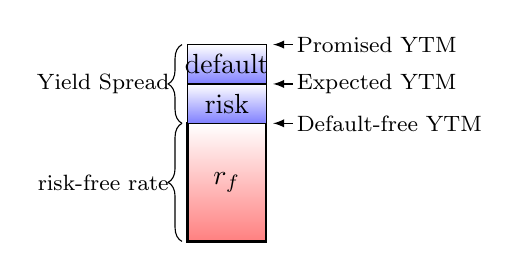
\begin{tikzpicture}[scale=0.5]
	%\draw[thick] (-1,0) rectangle +(11,6);
	\filldraw[thick, top color=white,bottom color=red!50!] (3.5,0.5) rectangle node{$r_f$} +(2,3);
	\filldraw[top color=white,bottom color=blue!50!] (3.5,3.5) rectangle node{risk} +(2,1);
	\filldraw[top color=white,bottom color=blue!50!] (3.5,4.5) rectangle node{default} +(2,1);
	\draw [decorate,decoration={brace,amplitude=5pt},xshift=-4pt,yshift=0pt]
	(3.5,0.5) -- (3.5,3.5) node [black,midway,xshift=-1cm] 
	{\footnotesize risk-free rate};
	\draw [decorate,decoration={brace,amplitude=5pt},xshift=-4pt,yshift=0pt]
	(3.5,3.5) -- (3.5,5.5) node [black,midway,xshift=-1cm] 
	{\footnotesize Yield Spread};
	
	\draw [-latex, ,xshift=5pt, right](6,3.5)--(5.5,3.5) node [right, ,xshift=5pt] {\footnotesize Default-free YTM};
	\draw [-latex, ,xshift=5pt, right](6,4.5)--(5.5,4.5) node [right, ,xshift=5pt] {\footnotesize Expected YTM};
	\draw [-latex, ,xshift=5pt, right](6,5.5)--(5.5,5.5) node [right, ,xshift=5pt] {\footnotesize Promised YTM};
\end{tikzpicture}

